\subsection{\label{sec:A2}Application to a nanorod sample}
As discussed in Section \ref{sec:aufbau}, dark-field spectra in the first diffraction 
order are recorded for all sample fields. 
In this process, the incident light is unpolarized or linearly polarized parallel or perpendicular 
to the longitudinal direction of the nanorods. 
Additionally, the spectrum of the illumination unit is recorded for each polarization, 
as well as the spectrum without any illumination, representing the background signal. 
The additionally recorded spectra are depicted in Figure \ref{fig:lampe}.
\begin{figure}[h!]
    \centering
    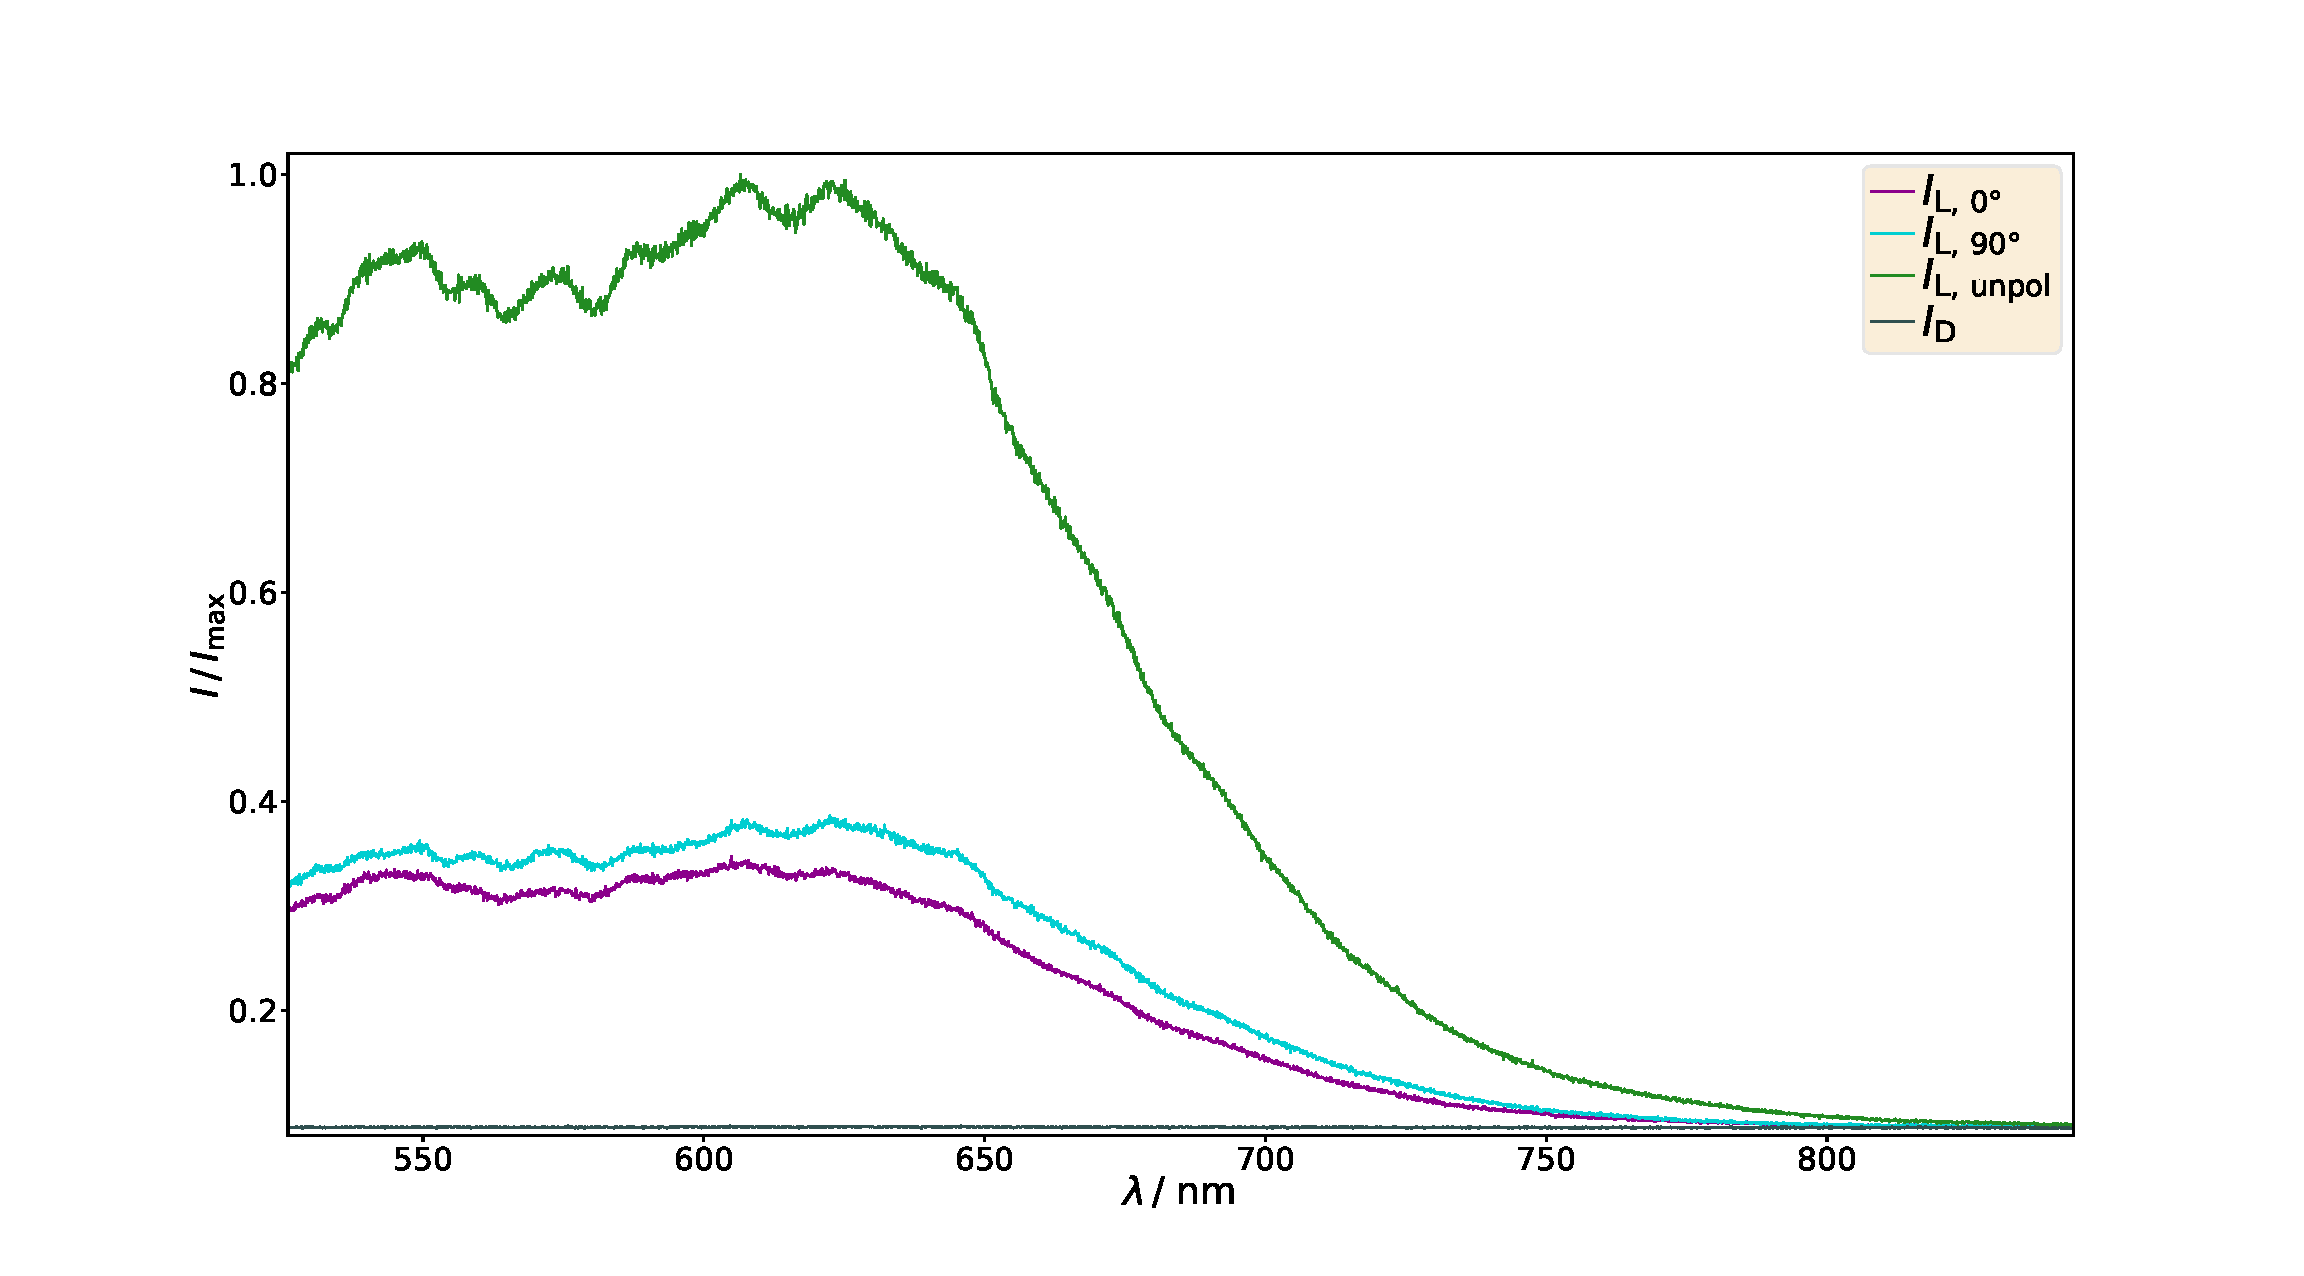
\includegraphics[clip, trim=3cm 1cm 3cm 2cm,width=0.85\textwidth]{Lampe.pdf}
    \caption{\label{fig:lampe}The lamp spectrum in various polarization settings, 
    along with the background signal captured without any illumination.}
\end{figure}\FloatBarrier
Since the lamp spectrum undergoes significant changes as a function of wavelength, 
this modulation needs to be divided out from the measured data. 
Additionally, the constant background signal must be subtracted, resulting in a corrected 
dark-field spectrum according to Eq.~\eqref{eq:korr}. 
As the lamp spectrum subtracted by the background signal approaches zero for large wavelengths, 
division is associated with a significant degradation of the signal-to-noise ratio. 
To address this for subsequent quantitative analyses, the respective intensities 
are smoothed before computation. \\
In Figure \ref{fig:spektren1}, the measured dark-field spectra for different sample 
fields and various light polarizations are presented. 
It should be noted that the displayed intensities have not been corrected for the background signal.
It therefore applies
\begin{equation}
    I_{\text{C}} = \frac{I_{\text{M}}}{I_{\text{L}}},
\end{equation} 
which means that the signal-to-noise ratio is better, since for long wavelengths 
$I_{\text{L}}$ approaches $I_{\text{D}}$.
The measured spectra are normalized to the most intense result to facilitate an intensity comparison.
\begin{figure}[h!]
    \centering
    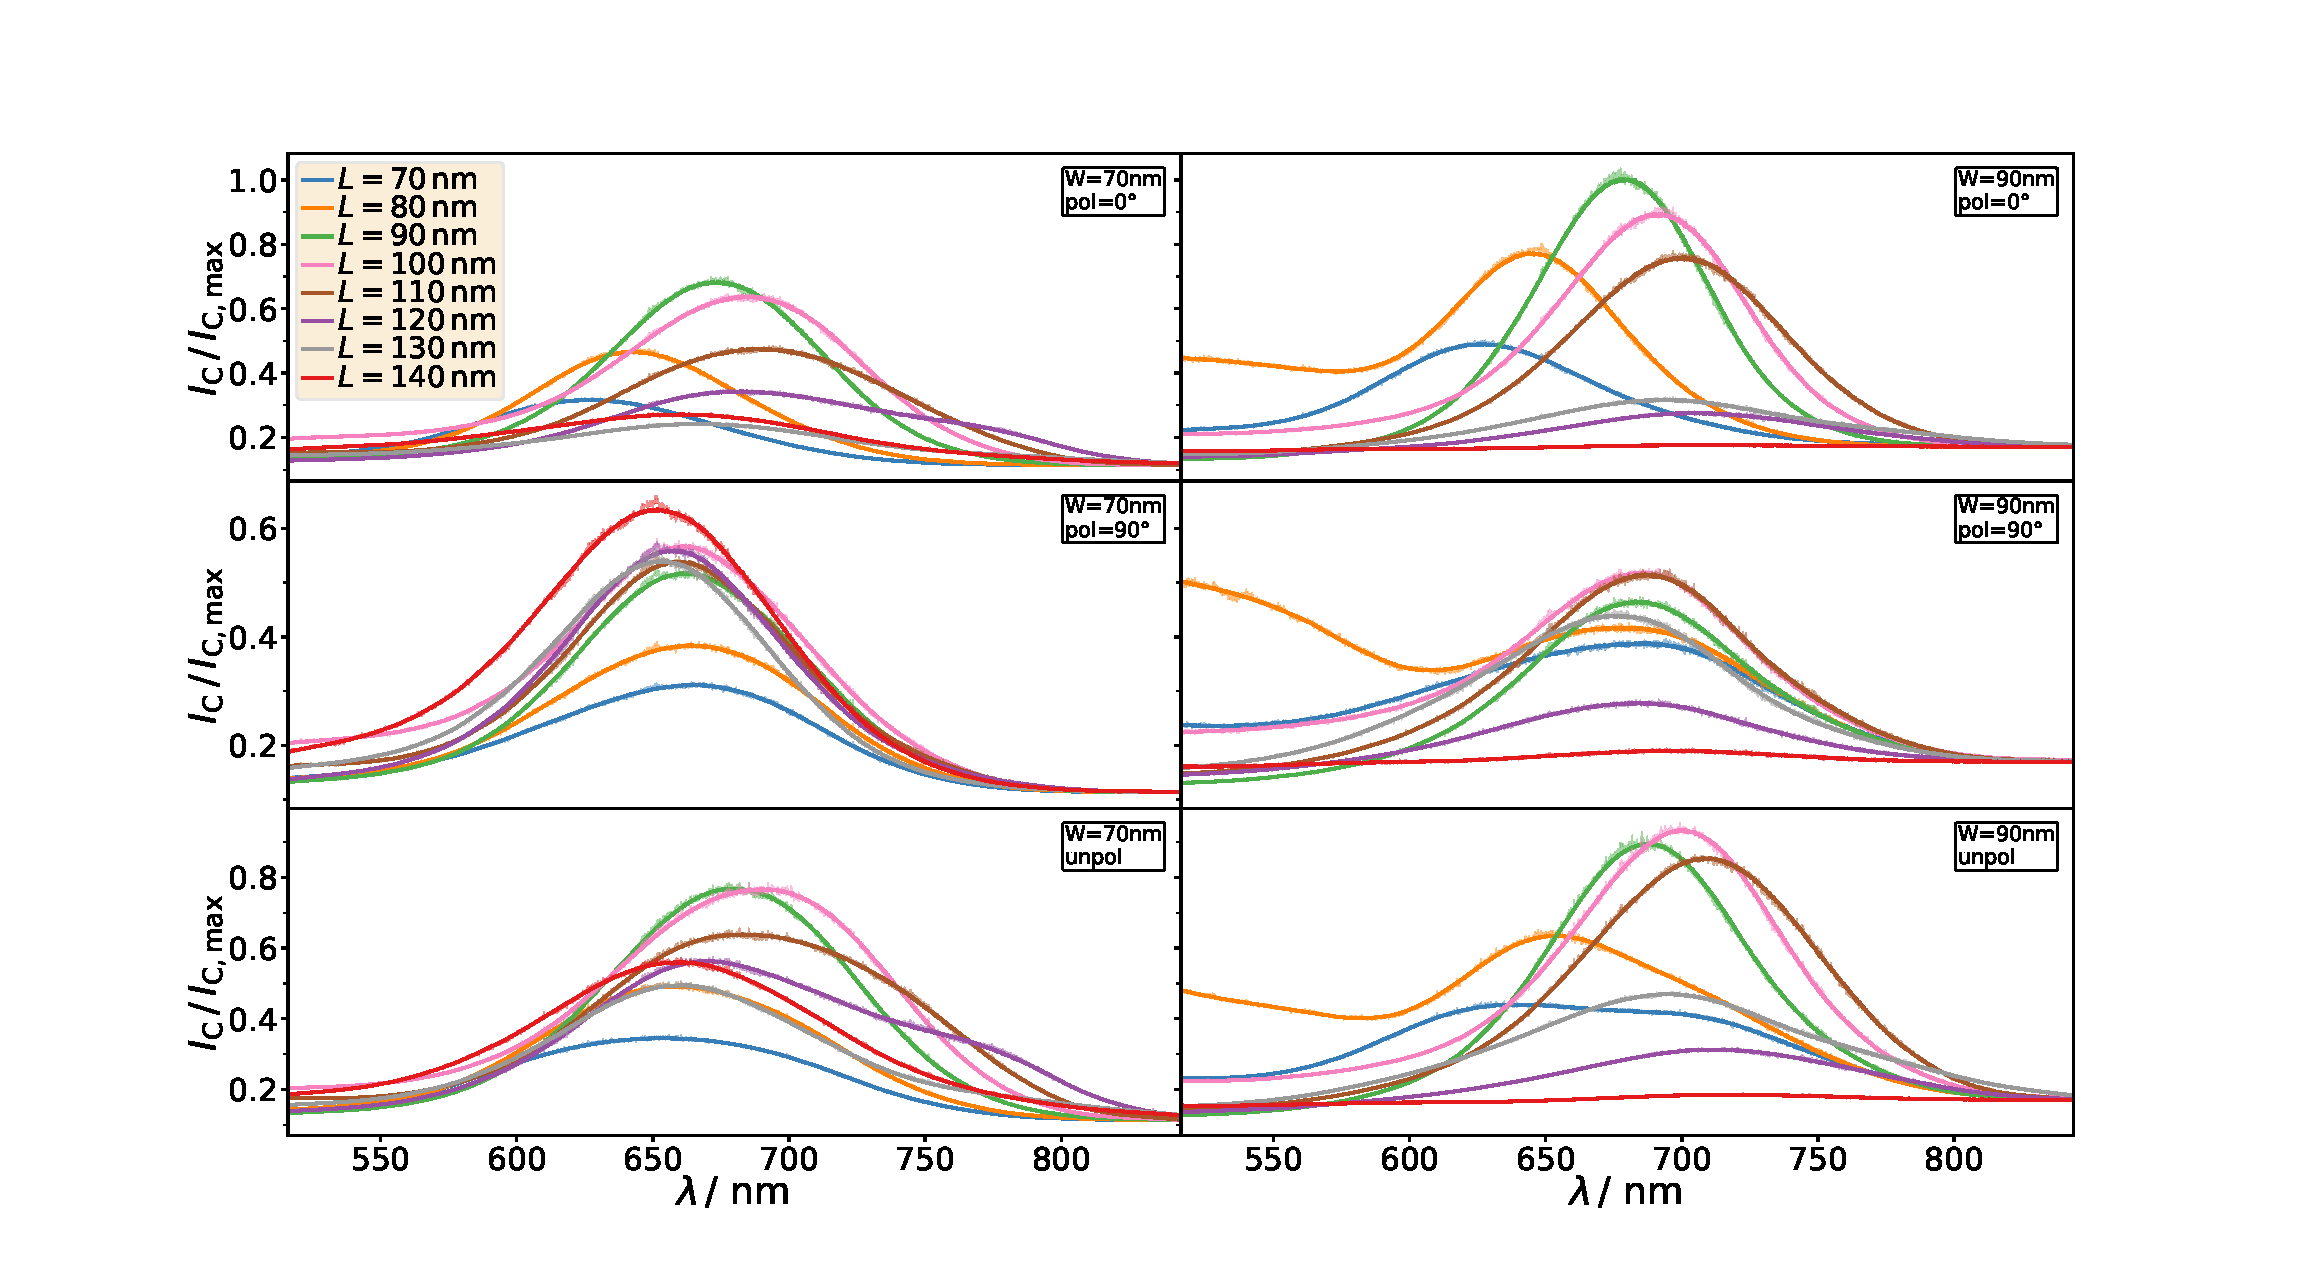
\includegraphics[clip, trim=3cm 1cm 3cm 2cm,width=\textwidth]{A2SpektrumsFalsch.pdf}
    \caption{\label{fig:spektren1}
    The measured dark-field spectra for different sample fields normalized to the strongest 
    intensity. 
    The left column depicts the upper sample group with a constant width of $W=70,\si{nm}$, 
    while the right column corresponds to the group with $W=90,\si{nm}$. Different rows 
    represent varying light polarizations, as indicated by the text box in the upper right corner. 
    Various colors in the plot correspond to different rod lengths $L$. Both the unsmoothed 
    and smoothed signals are presented. It is important to note that the current view employs 
    an incorrect intensity correction, yielding deceptively good results that are, however, inaccurate.}
\end{figure} \FloatBarrier
While this visually yields a pleasing result, it is not suitable for analyses as 
the resonance wavelength is inaccurately determined from it. \\
Applying the correction formula correctly, the spectra are depicted according to 
Eq.~\eqref{eq:korr} in Figure \ref{fig:spektren2}.
\begin{figure}[h!]
    \centering
    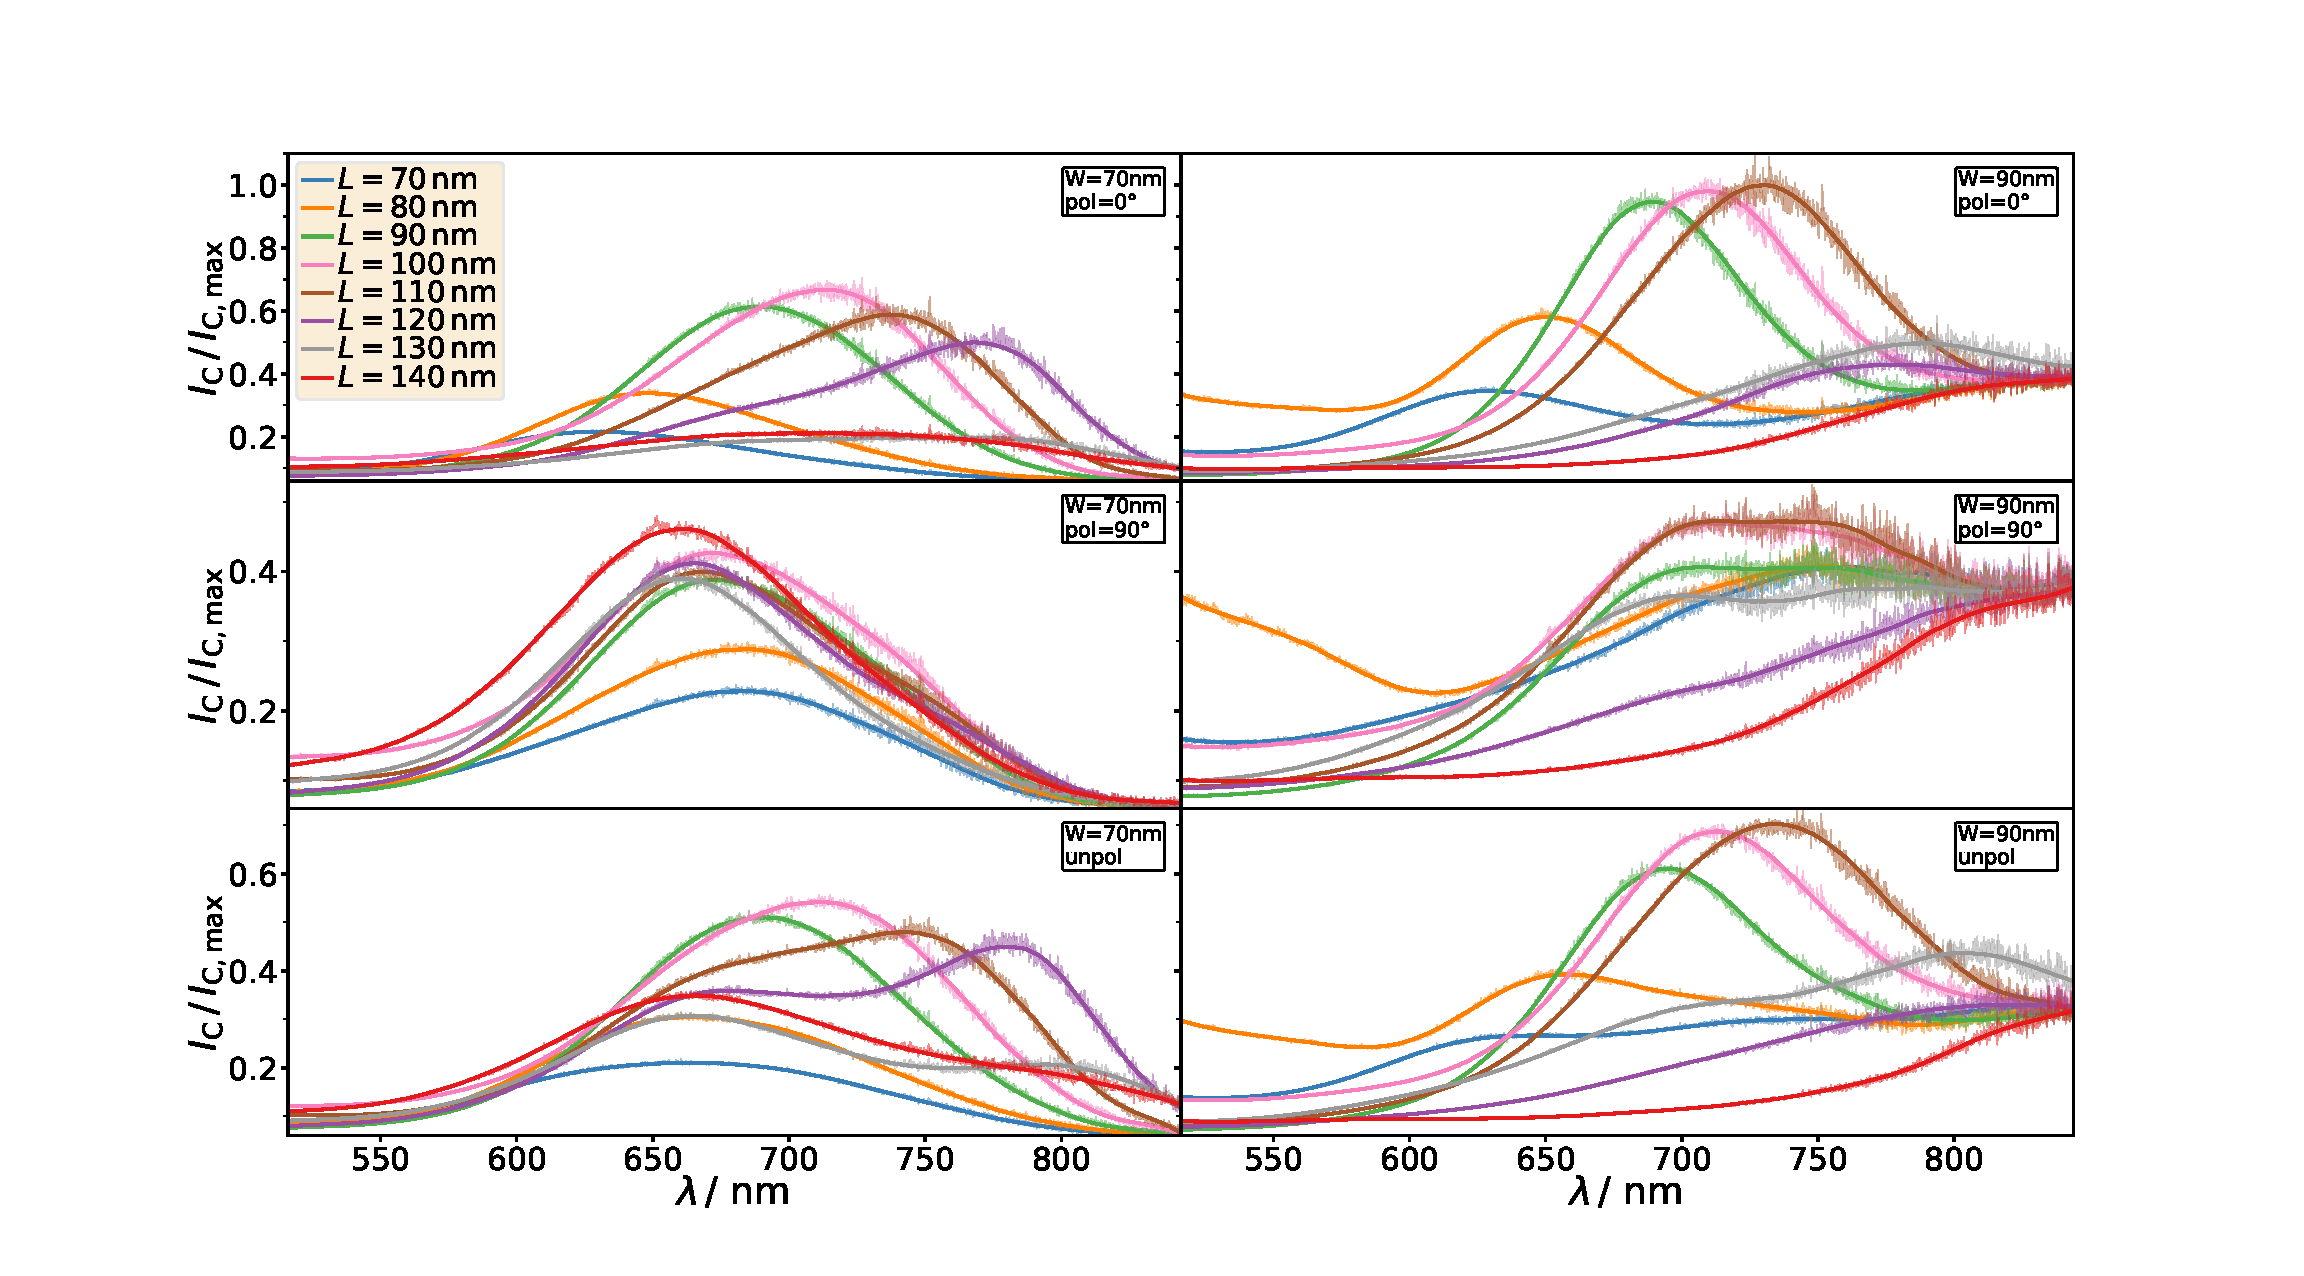
\includegraphics[clip, trim=3cm 1cm 3cm 2cm,width=\textwidth]{A2Spektrums.pdf}
    \caption{\label{fig:spektren2}The correctly corrected measurement values as a function of wavelength. 
    The graphical layout remains unchanged compared to the previous plot. 
    The only difference is that the constant background signal is subtracted from the lamp 
    spectrum and the measurement spectrum before dividing them.}
\end{figure} \FloatBarrier
It is clearly evident that the signal-to-noise ratio deteriorates, 
but this is effectively mitigated by the smoothing of the values. 
Additionally, based on the wavelength peaks at $0^{\circ}$ polarization angle, 
it can be observed that the shift is more pronounced compared to Figure \ref{fig:spektren1}. \\ \\
Before delving into the further analysis of the resonance wavelength shift, 
let's first examine the measured dark-field spectra from Figure \ref{fig:spektren2}. 
Initially, it is noticeable that for a polarization angle of $\alpha=0^{\circ}$, 
the peaks that emerge are significantly shifted, with a stronger shift for longer nanorods in the sample. 
This shift is attributed to the enlargement of the resonator, leading to a displacement 
of the resonance wavelength. 
For a perpendicular polarization, this shift is not observed, as expected. 
However, it can be observed that the peak for $W=70\,\si{nm}$ is around $\lambda\approx 680\,\si{nm}$. 
For $W=90\,\si{nm}$, this resonance wavelength of the transverse plasmon mode seems to shift 
slightly to longer wavelengths. 
However, the noise in the signal increases significantly here, as the measurement signal 
is divided by very small values for large wavelengths. \\
In the last row, the nanorod samples are excited with unpolarized light, 
hence occasionally two peaks are visible, as both transverse and longitudinal plasmon modes can be excited. 
However, the resolution is finest for parallel polarization, where our analysis will be continued. \\ \\
By performing a Gaussian fit, the intensity maxima of the measurement with $\alpha = 0^{\circ}$ are 
associated with a wavelength. For this purpose, only the smoothed measurement values are considered, 
and the Gaussian function is fitted only around the center of the maximum. 
This is necessary because the measured spectra often do not exhibit an ideal Gaussian shape, 
leading to a significant deterioration of the fitting result. The presentation of the fits is 
intentionally omitted, as no new insights are gained, and the maximum intensity can essentially 
be read from Figure \ref{fig:spektren2}. 
The relevant measured parameter $\mu$ of the 
fitted function $G(\lambda) = A\exp\left(-\frac{(\lambda-\mu)^{2}}{2\sigma^{2}}\right)$ is tabulated 
in Table \ref{tab:daten}. 
The shift $\mu$ corresponds to the resonance wavelength $\lambda_{\text{R}}$, and its error arises from
the applied fitting algorithm and an estimated amplification factor 
resulting from signal smoothing and a non-ideal gaussian shape of the signal. \\
TABELLE \\ \\

With Eq.~(2.5) from the experimental manual \cite{Anleitung}, 
by plotting the resonance wavelengths against the resonator length $L$ of the nanorods, 
the effective refractive index of the plasmons $n_{\text{eff}}$ and the extension of the 
resonator $\Delta{L}$ can be determined. The relation is given by
\begin{equation}
    \lambda_{\text{R}} = 2n_{\text{eff}}L + 2\Delta{L}.
\end{equation}
Fitting a straight line to the plotted values allows the desired parameters 
to be calculated from the slope and intercept. \\
In Figure \ref{fig:lin}, the measured values, errors, and the fitted lines for sample 
groups of different widths are presented.
\begin{figure}[h!]
    \centering
    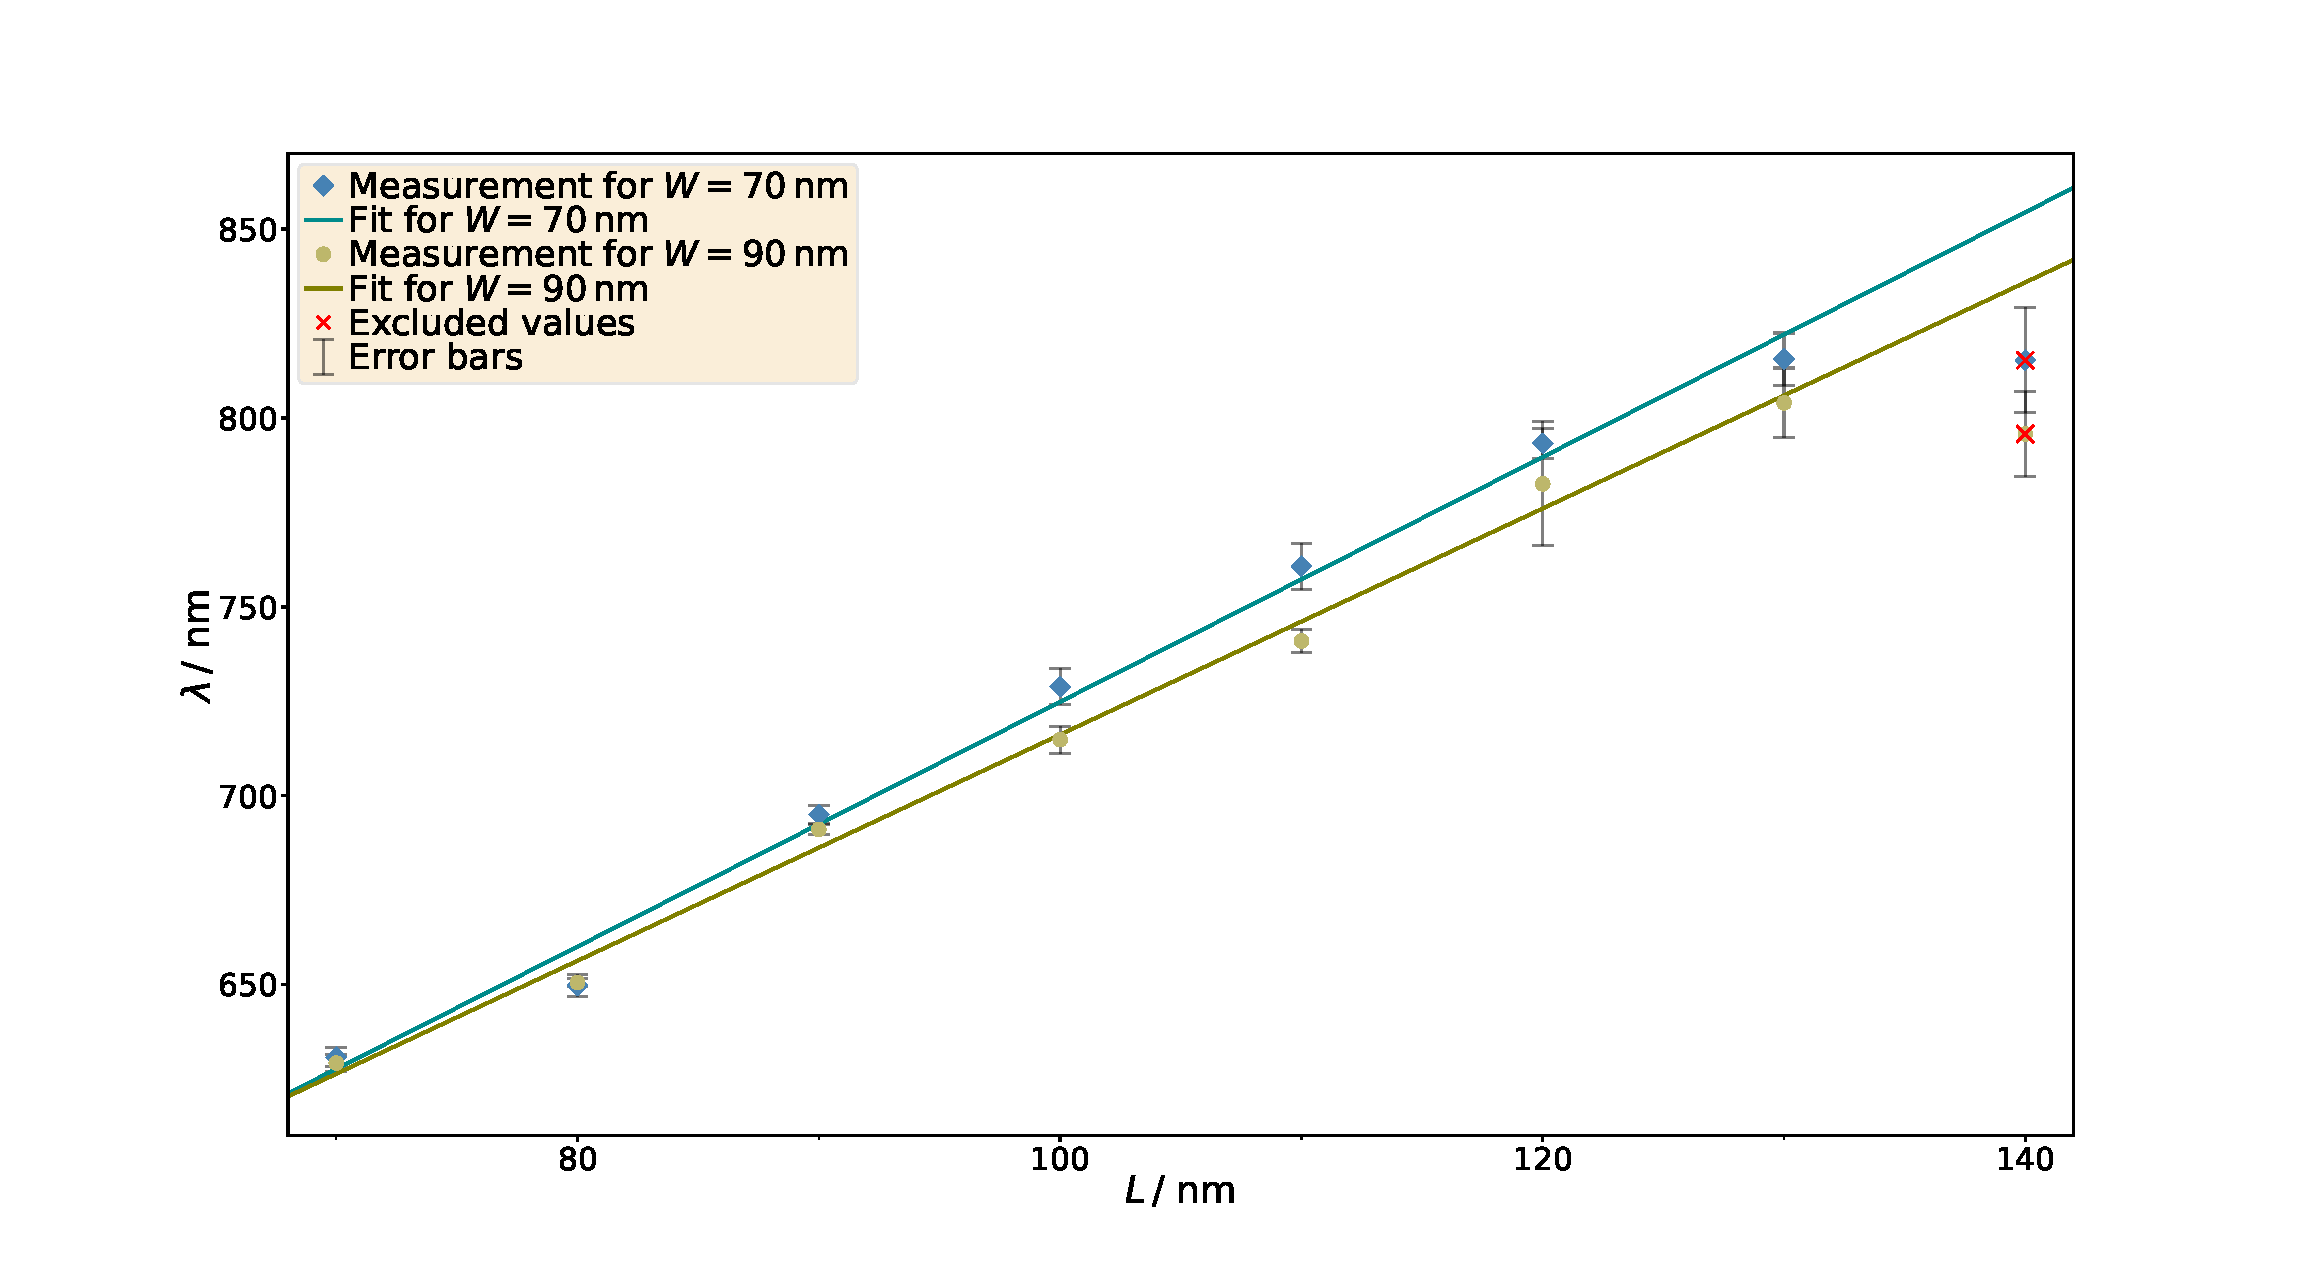
\includegraphics[clip, trim=3cm 1cm 3cm 2cm,width=\textwidth]{A2Fit.pdf}
    \caption{\label{fig:lin}}
\end{figure}\FloatBarrier

Kurz Diskussion der Messwerte, sowie ausschluss der jeweils letzten Werte. 
Dann auflistung der seperierten Ergebnisse, dann Mittelwert in Kasten. 
Die Ergebnisse kurz Besprechen und Plausifizieren, dann 
Abschluss und Fazit schreiben. 








